\clearpage
\section{Phase 6: Legal Abstractive Summarization}
\label{sec:phase6}

\subsection{Task, constraints and evaluation}
The system receives a judgment and must compress its material facts, legal
reasoning and disposition into a readable abstraction. Given a document
\(d\) and output tokens \(y_{1:m}\), a conditional generator models
\[
 p_\theta(y_{1:m}\mid d)=\prod_{t=1}^{m}p_\theta(y_t\mid d,y_{<t}).
\]
For long cases the submitted system applies this factorization separately to
selected passages of \(d\), then orders and merges their outputs. This trades
whole-document context for multiple bounded generation calls. An abstraction
can paraphrase beyond source sentences, so factual support and lexical overlap
are separate questions. See \href{https://arxiv.org/abs/1904.09675}{Zhang et al. on BERTScore}.

The course required adaptation of all four Phase~1 architectures, including
LoRMA and a smaller distilled model. Training was confined to the course
dataset and the project's own Phase~1 weights. The official configuration,
\path{Phase_6_Summ}, provides \path{Train/train.json} and \path{Test/test.json}.
The labeled records contain an ID, judgment and summary. Test references are
hidden, and the course publishes no separate development split. Each submitted
archive contains a root-level \path{prediction.json} with an ID and a nonempty
summary per test judgment. The course specifies \BERT{} as the primary measure
and ROUGE-1/ROUGE-L F1 as secondary measures. The available official result
record contains the primary scores and submission IDs. Local results are
mean stemmed ROUGE F1 over held-out judgments and are reported separately.

\subsection{Data and the context constraint}
Of 7,030 labeled records, 6,466 went to training and 564 to validation. A
grouped split uses SHA-256 of whitespace-normalized source text to keep exact
duplicates together. The archived partition is authoritative for replay.
The 100 test judgments were reserved for submission. The original notebook
reports a median of 17,905 source characters, rising to 45,052 at the 90th
percentile. References have a median of 638 words, a 90th percentile of
1,501 and a maximum of 27,768. Two training references are empty.
The original 240-token target cap includes the end-of-sequence token and
already binds at the median training example. The original and revised
methods therefore solve substantially different supervision problems.

\begin{figure}[!htb]
\centering
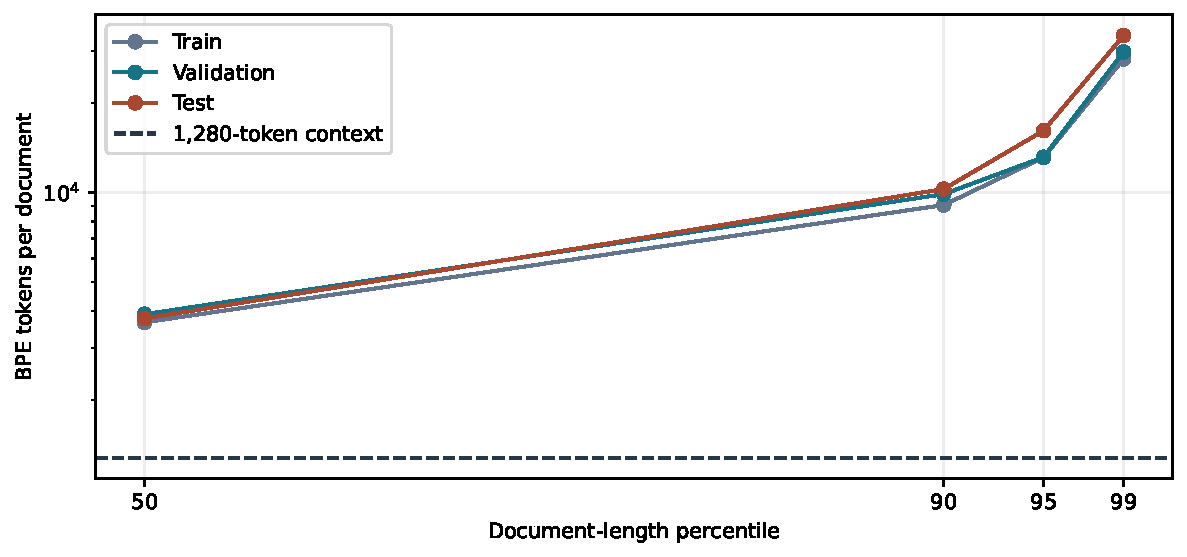
\includegraphics[width=.84\linewidth]{figures/phase6/p6_data_lengths.pdf}
\caption{Document length quantiles obtained with the archived 32k Phase~1
byte-level BPE tokenizer. The dashed line marks the causal context budget
before accounting for prompt or output tokens.}
\label{fig:p6-lengths}
\end{figure}

The split-level measurements in Table~\ref{tab:p6-lengths} show that even
the median document is almost three times the causal context. The training
reference itself has a median of 753 BPE tokens, beyond either target cap.
The 99th-percentile training source has 28,190 BPE tokens, with a maximum of
162,070. The median within-case document-to-summary ratio is 4.59:1 for
nonempty training references and 4.65:1 in validation. The labeled file
contains 27 extra rows beyond its number of normalized-text groups. No
labeled and test IDs or exact normalized sources overlap. Exact hashing
does not detect edited near duplicates.

\begin{table}[!htb]
\centering\small
\caption{Median source and reference lengths. Source thresholds use the 1,280-token
causal context before prompt or output tokens. Test references are private.}
\label{tab:p6-lengths}
\begin{tabular}{lrrrrr}
\toprule
Split & Count & Source words & Source BPE & Over context & Ref. words \\
\midrule
Train & 6,466 & 3,120 & 3,657 & 94.4\% & 638 \\
Validation & 564 & 3,353 & 3,893 & 93.1\% & 647 \\
Test & 100 & 3,171 & 3,768 & 95.0\% & -- \\
\bottomrule
\end{tabular}
\end{table}

\subsection{Inputs, alignment and training coverage}
\paragraph{Original section packing.}
The notebook divides a long judgment into 150-token sections, prioritizes the
first and last two sections, then ranks the remaining sections by legal-term
frequency with a small bonus for later position. It concatenates the selected
sections in source order under a nominal 900-token text budget, with a single
instruction and summary cue. The target takes up to 239 BPE tokens and appends
EOS, even if the last reference sentence is incomplete. The training cache
contains one pair per judgment. A head-only comparator replaces the section
selection with the initial source span. The method packs discontiguous
evidence into one context and gives the model a single output budget.

\paragraph{V2 passage alignment.}
The revisions use contiguous 840-token windows. The first and last windows
are mandatory, with up to two interior windows chosen by legal-term frequency
and a decision-cue bonus. The prompt labels each selected passage by its
position among the selected passages. During training, for each reference
sentence \(s\) and passage \(p\) the assignment score is
\[
 a(s,p)=\frac{|W(s)\cap W(p)|}{\max(1,\sqrt{|W(s)||W(p)|})},
\]
where \(W\) is the set of lowercased content words and eligible numerals.
The best passage receives the sentence if its score reaches 0.05. V2 forms
one target of up to 319 tokens plus EOS per eligible passage, preferring
high-overlap sentences when the assigned text exceeds the budget. Selection
for inference depends only on the source. The cache has 21,710 training
passage examples across 6,464 usable judgments and 1,897 validation passages.
Each epoch rotates one passage per judgment, yielding 19,392 draws over
three epochs with repeated passages on shorter cases and omissions for
cases with four targets.

\paragraph{V3 target packing.}
V3 preserves the order of all aligned sentences and opens a new target pack
when the next sentence would exceed the cap. It tries clause boundaries for
overlong sentences and skips fragments that still cannot fit. Sentences
without a qualifying passage remain outside the training targets. V3 draws
31,668 packed targets, or 4.9 per usable training judgment, plus 2,778
validation targets. The 50th, 90th and 99th percentiles of training target
length including EOS are 212, 309 and 319. Each run shuffles judgments,
shuffles their target packs and visits all packs once, resulting in 7,917
optimizer updates. The evidence establishes complete coverage of the
materialized target set.

\subsection{Backbones, parameter updates and objective}
All adaptations reuse the Phase~1 32k BPE, with PAD, BOS, EOS and UNK at IDs
0 through 3. The GQA runs start from the 700M-token foundation. The other
backbones use their Phase~1 best snapshots. The encoder--decoder attends
bidirectionally to an input of up to 1,024 tokens, and generates with a
causal decoder of capacity 640 with cross-attention. Prefix-LM processes its
source prefix bidirectionally and continues causally, within 1,280 tokens.
The standard decoder uses causal self-attention and learned positional
embeddings. Efficient GQA is causal with fourteen 768-wide blocks, twelve
query and four KV heads, rotary position embeddings, RMS normalization and
SwiGLU. See \href{https://aclanthology.org/2023.emnlp-main.298/}{Ainslie et al. on grouped-query attention}. The GQA LoRA run trains 3.06M of its 115.72M parameters in V3.

\begin{itemize}[leftmargin=*]
\item E01 and E05 test additive low-rank adaptation on encoder--decoder and
Efficient GQA. A frozen projection \(W\) receives the trainable update
\(Wx+(\alpha/r)BAx\).
\item E02 tests the notebook's LoRMA+ multiplicative form. If \(z=Wx\), the
layer returns \(z+(\alpha/r)BAz\). Its low-rank factors operate in the
projection's output space.
\item Original low-rank adapters have rank 8 and scale \(\alpha/r=2\).
They target selected attention projections. V2/V3 use rank 16 and the same
scale, expand adaptation to attention and MLP linears, and train the
normalization parameters.
\item E03 tests a prefix-conditioned source with residual adapters. The
original attaches a normalized width-64 ReLU adapter after the block.
V2/V3 insert separate bottlenecks after attention and the MLP and also train
the layer norms. Up-projections start at zero.
\item E06 trains all 101.97M encoder--decoder parameters. E04 and E07 train
all 82.26M parameters of an eight-layer causal student assembled from layers
0, 2, 3, 5, 6, 8, 9 and 11 of the Phase~1 standard decoder.
\end{itemize}

The adaptation designs follow
\href{https://arxiv.org/abs/2106.09685}{Hu et al. on LoRA},
\href{https://arxiv.org/abs/2506.07621}{the LoRMA paper} and
\href{https://proceedings.mlr.press/v97/houlsby19a.html}{Houlsby et al. on adapters}.
The formulas above describe this project's implemented variants.

Teacher forcing minimizes mean target-token cross-entropy
\[
 \mathcal L_{\mathrm{CE}}=-\frac{1}{|y|}\sum_{t=1}^{|y|}
 \log p_\theta(y_t\mid x,y_{<t}).
\]
EOS is supervised. Decoder-only and prefix models use logits starting at the
last prompt position, masking source positions out of the loss by slicing.
The encoder--decoder sees the source in the encoder and BOS followed by
shifted gold tokens in its decoder. Microbatches contain one example, avoiding
padding masks. The optimizer is AdamW with weight decay 0.01, accumulation
over four examples and gradient clipping at 1.0. The notebooks use mixed
precision, warm-up and cosine decay. Original updates range from 500 to
800. V2 uses 4,848 updates per run. V3 uses one complete 7,917-update pass.
Learning rates decrease from \(2\cdot10^{-4}\) for original adapters, to
\(1.5\cdot10^{-4}\) for V2 and \(8\cdot10^{-5}\) for V3. Full fine-tuning
uses \(2\cdot10^{-5}\) in original/V2 and \(10^{-5}\) in V3.
Student rates are \(4\cdot10^{-5}\) in original/V2 and \(2\cdot10^{-5}\) in V3.

\subsection{Teacher and student comparison}
E02 was the teacher in each version. The original selects the teacher by
held-out ROUGE-L and generates responses for 1,000 documents. V2 selects
by hierarchical ROUGE-1 and stores 2,686 generated passage responses from
800 selected judgments. In both, approximately half of E04's scheduled draws
are replaced by draws from the teacher-labeled pool. For examples with a
pseudo-target, the original mixes gold and teacher-sequence CE equally.
V2 uses a 60:40 gold-to-teacher mixture. V2 E04 reaches 0.3160 local ROUGE-1
against 0.3976 for its gold-only counterpart.

V3 uses the V2 gold-only checkpoint as the initialization for both E04 and
E07. The larger frozen E02 teacher receives the same gold target prefix as
the student and computes the vocabulary distributions online. With
\(p_T\) the teacher distribution and \(q_T\) the student distribution at
temperature \(T=2\), the loss is
\[
  \mathcal L_{\mathrm{V3,E04}} =
  0.8\,\mathcal L_{\mathrm{CE}}+
  0.2\, T^2\,\frac{1}{|y|}\sum_{t=1}^{|y|}
  D_{\mathrm{KL}}\!\left(p_T(\cdot\mid x,y_{<t})
        \,\|\,q_T(\cdot\mid x,y_{<t})\right).
\]
E07 uses gold CE alone. The controls share architecture, warm start, budget
and coverage. Run-specific shuffles differ. E04 improves held-out NLL over
E07 (2.3575 versus 2.3768), while E07 leads it by 0.0259 in validation
ROUGE-1 and 0.0017 in official \BERT{}. The data support the outcome of this
one teacher, temperature and mixture with their observed shuffles. The
smaller V3 ROUGE gap relative to V2 is descriptive, since data construction,
training budget and evaluation sample changed.

\subsection{Decoding, selection and results}
Original cached greedy decoding blocks PAD, BOS, UNK and repeat trigrams,
uses a repetition penalty of 1.12 and allows EOS after 40 generated tokens,
with a 192-token cap. V2/V3 use 1.10, 32 and 260 respectively, per selected
passage and within context capacity. They trim a trailing incomplete segment
when the last terminal punctuation is at or after 65\% of the generated
text, then combine passages in document order. Sentence deduplication drops
later candidates with content-word Jaccard overlap above 0.73. This merge
preserves more separate source evidence and can retain contradictions across
passages.

V3 compares raw merging with an optional lexical filter. A sentence must
share at least 52\% of its eligible words with the source and any matched
multi-digit number must occur in the source text. If fewer than 30 words
survive deduplication, it falls back to the raw summary. All seven V3
experiments selected raw based on held-out ROUGE-1. For E05 the filter
reduces mean length from 295 to 273 words and ROUGE-1 from 0.4092 to
0.3931. This proxy can remove valid paraphrases and retain reversed legal
relationships with shared vocabulary.

\begin{figure}[!htb]
\centering
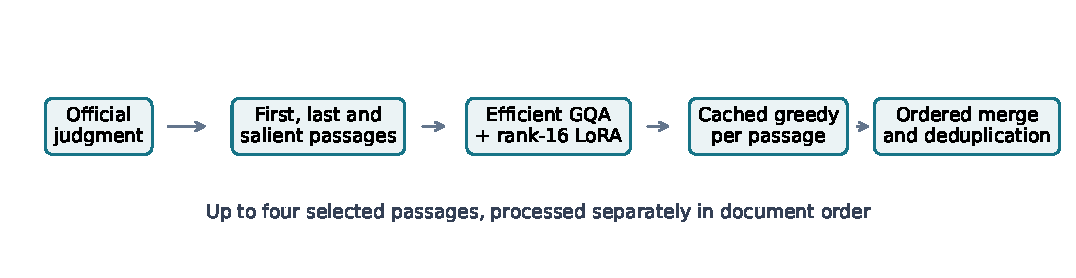
\includegraphics[width=.97\linewidth]{figures/phase6/p6_e05_pipeline.pdf}
\caption{Submitted E05 inference. Passage selection precedes cached generation.
The raw policy orders and deduplicates generated sentences.}
\label{fig:p6-pipeline}
\end{figure}

\begin{table}[!htb]
\centering\small
\caption{V3 held-out and official results. Local scores use 96 documents.
Official scores use 100 hidden-reference cases. IDs and scores are transcribed
from the supplied Codabench screenshot and mapped by the submission order.}
\label{tab:p6-official}
\begin{tabular}{llrrrrr}
\toprule
Run & Method & Best step & ROUGE-1 & ROUGE-L & \BERT{} & ID \\
\midrule
E01 & Enc.--dec. LoRA & 7,917 & .2504 & .1602 & .8217 & 1026549 \\
E02 & GQA LoRMA & 7,917 & .4129 & .2278 & .8442 & 1026551 \\
E03 & Prefix Houlsby & 7,750 & .2847 & .1764 & .8239 & 1026552 \\
E04 & Causal student KL & 7,750 & .3975 & .2198 & .8438 & 1026554 \\
E05 & GQA LoRA & 7,750 & .4092 & .2236 & \textbf{.8459} & 1026556 \\
E06 & Enc.--dec. full & 7,917 & .2686 & .1661 & .8232 & 1026558 \\
E07 & Causal student CE & 7,500 & \textbf{.4234} & \textbf{.2310} & .8455 & 1026559 \\
\bottomrule
\end{tabular}
\end{table}

\begin{figure}[!htb]
\centering
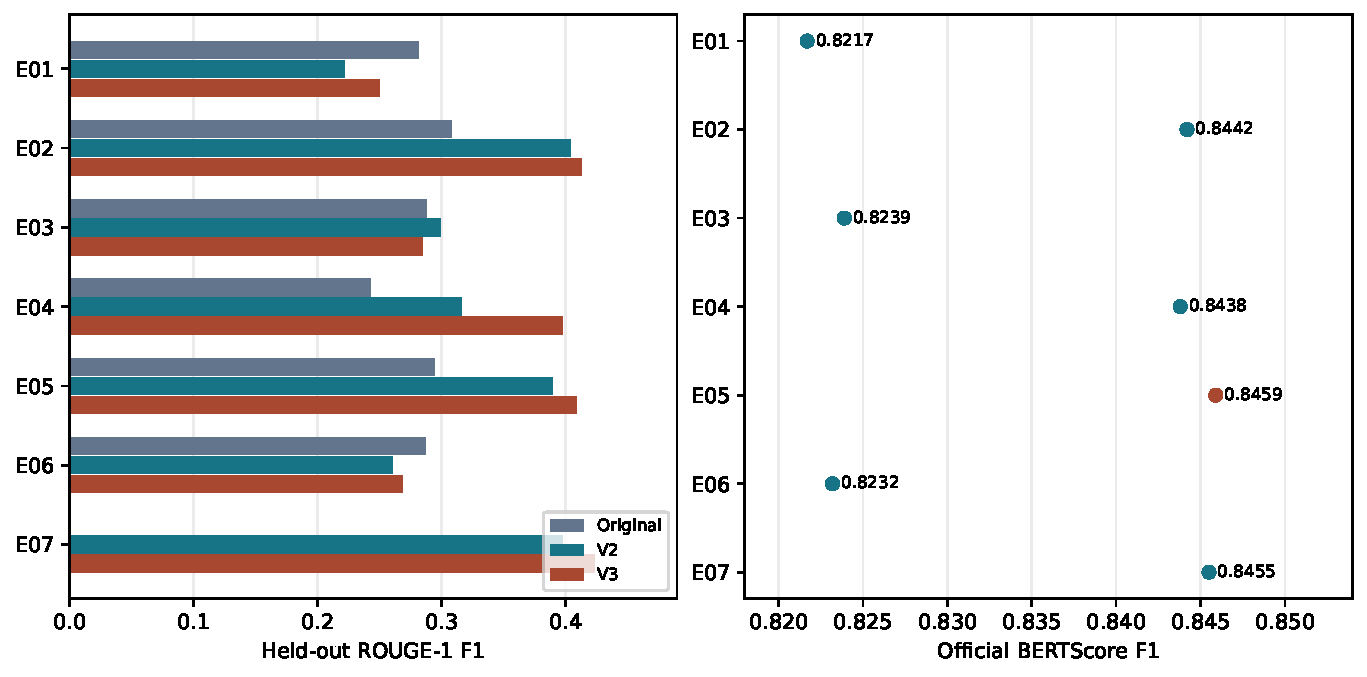
\includegraphics[width=.98\linewidth]{figures/phase6/p6_results.pdf}
\caption{Local lexical performance by revision and official V3 BERTScore F1.
Local samples contain 32, 64 and 96 judgments across the three revisions.
The two panels use different metrics and evaluation cases.}
\label{fig:p6-results}
\end{figure}

\begin{figure}[!htb]
\centering
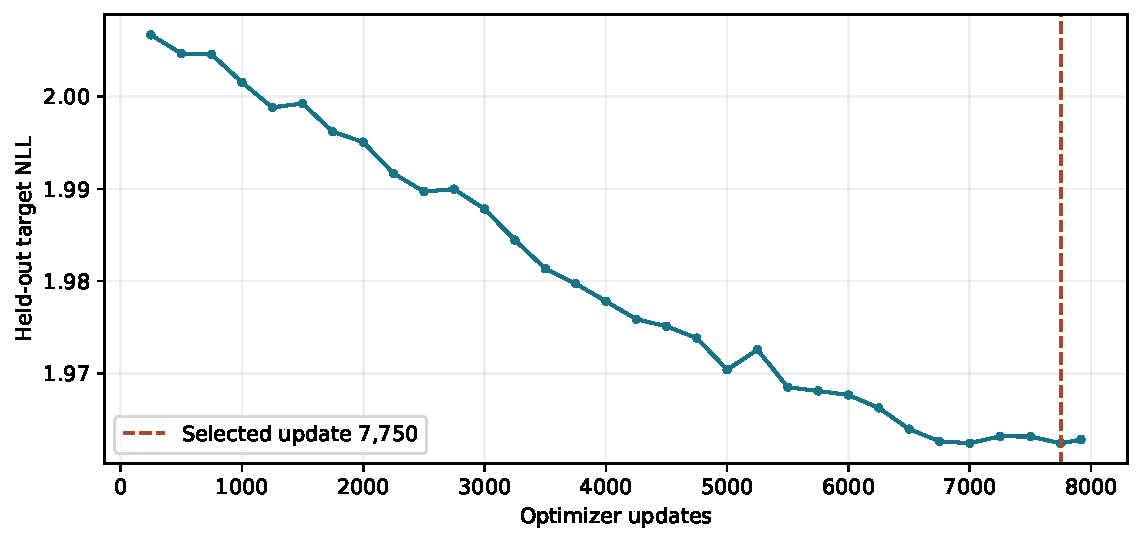
\includegraphics[width=.83\linewidth]{figures/phase6/p6_e05_history.pdf}
\caption{Archived V3 E05 target NLL on the fixed validation subset.
The archive selected update 7,750. Several late values look close at the
displayed precision. The selected update comes from the submission manifest.}
\label{fig:p6-history}
\end{figure}

\paragraph{Long-case ablation.}
On V2's matched 64 judgments and E02 weights, head-only decoding gives
0.1797 ROUGE-1 and hierarchical decoding 0.4042. With V3's matched 96
judgments, the raw scores are 0.1860 and 0.4129. In V3 the mean output
length also increases from 98 to 302 words. The comparison changes both
source access and the number of possible generation calls. It does not
isolate salience, document coverage or length as causes.

\paragraph{What changed across runs.}
Original E02 led its local comparison at 0.3081 ROUGE-1. V2's better
document coverage and revised supervision gave the GQA and distilled runs
higher measured ROUGE, while encoder--decoder runs moved in the opposite
direction on the changed validation sample. V3 added more supervision
per selected passage and resumed the V2 models. E03's V3 lexical scores
declined relative to V2, even with the larger passage schedule. On the V3
official set the two GQA adapters and two causal students scored between
0.8438 and 0.8459. E01, E03 and E06 scored from 0.8217 to 0.8239. Initialization,
attention structure and trainable layers differ, so this ranking cannot
isolate an architecture or adaptation effect. E05 is the official winner
among the seven project submissions. Its 0.0004 advantage over E07 does
not establish a generalization advantage without paired scores or repeat
runs.

\subsection{Qualitative errors and scope of verification}
In archived V2 E02 validation output for judgment 1770, the generated
text adds Section 307 alongside Section 302 and changes the account of the
appellate reasoning relative to the reference. In judgment 757, the
prediction introduces a \pounds2,000 figure absent from the reference
account of the pension arrangement. These examples show how legal-sounding
details can diverge from reference facts. The analysis is illustrative and
does not estimate error prevalence or prove absence from every source
passage. A candidate may also copy a correct number in the wrong role,
or omit the disposition if the selected windows or generation budgets
discard it.

The evidence audit validates the archived submissions against the official
test IDs, recomputes available held-out metrics from saved predictions and
checks the selected run against the V3 manifest. Model and optimizer tests
exercise the port on synthetic weights. The original E05 checkpoint exceeds
the available Drive transfer limit. Original-weight decoding, full GPU
training and private score recomputation remain outside the verification
performed here.

\subsection{Conclusion}
The best recorded official summary system combines Phase~1 Efficient GQA
with a small trainable LoRA component and reference-independent passage
selection. Multiple generation calls recover more lexical coverage than a
single head window in matched comparisons. The distilled student remained
competitive, but its gold-only control scored higher on both generated
validation summaries and the hidden test. For legal use, the archived
errors motivate separate factual checks beyond the primary metric.
